\documentclass[border=10pt]{standalone}

\usepackage{tikz}
\usepackage{tikzsymbols}
\usetikzlibrary{calc,patterns,shapes.geometric}

\def\centerarc[#1](#2)(#3:#4:#5){\draw[#1] ($(#2)+({#5*cos(#3)},{#5*sin(#3)})$) arc (#3:#4:#5);}

\begin{document}
	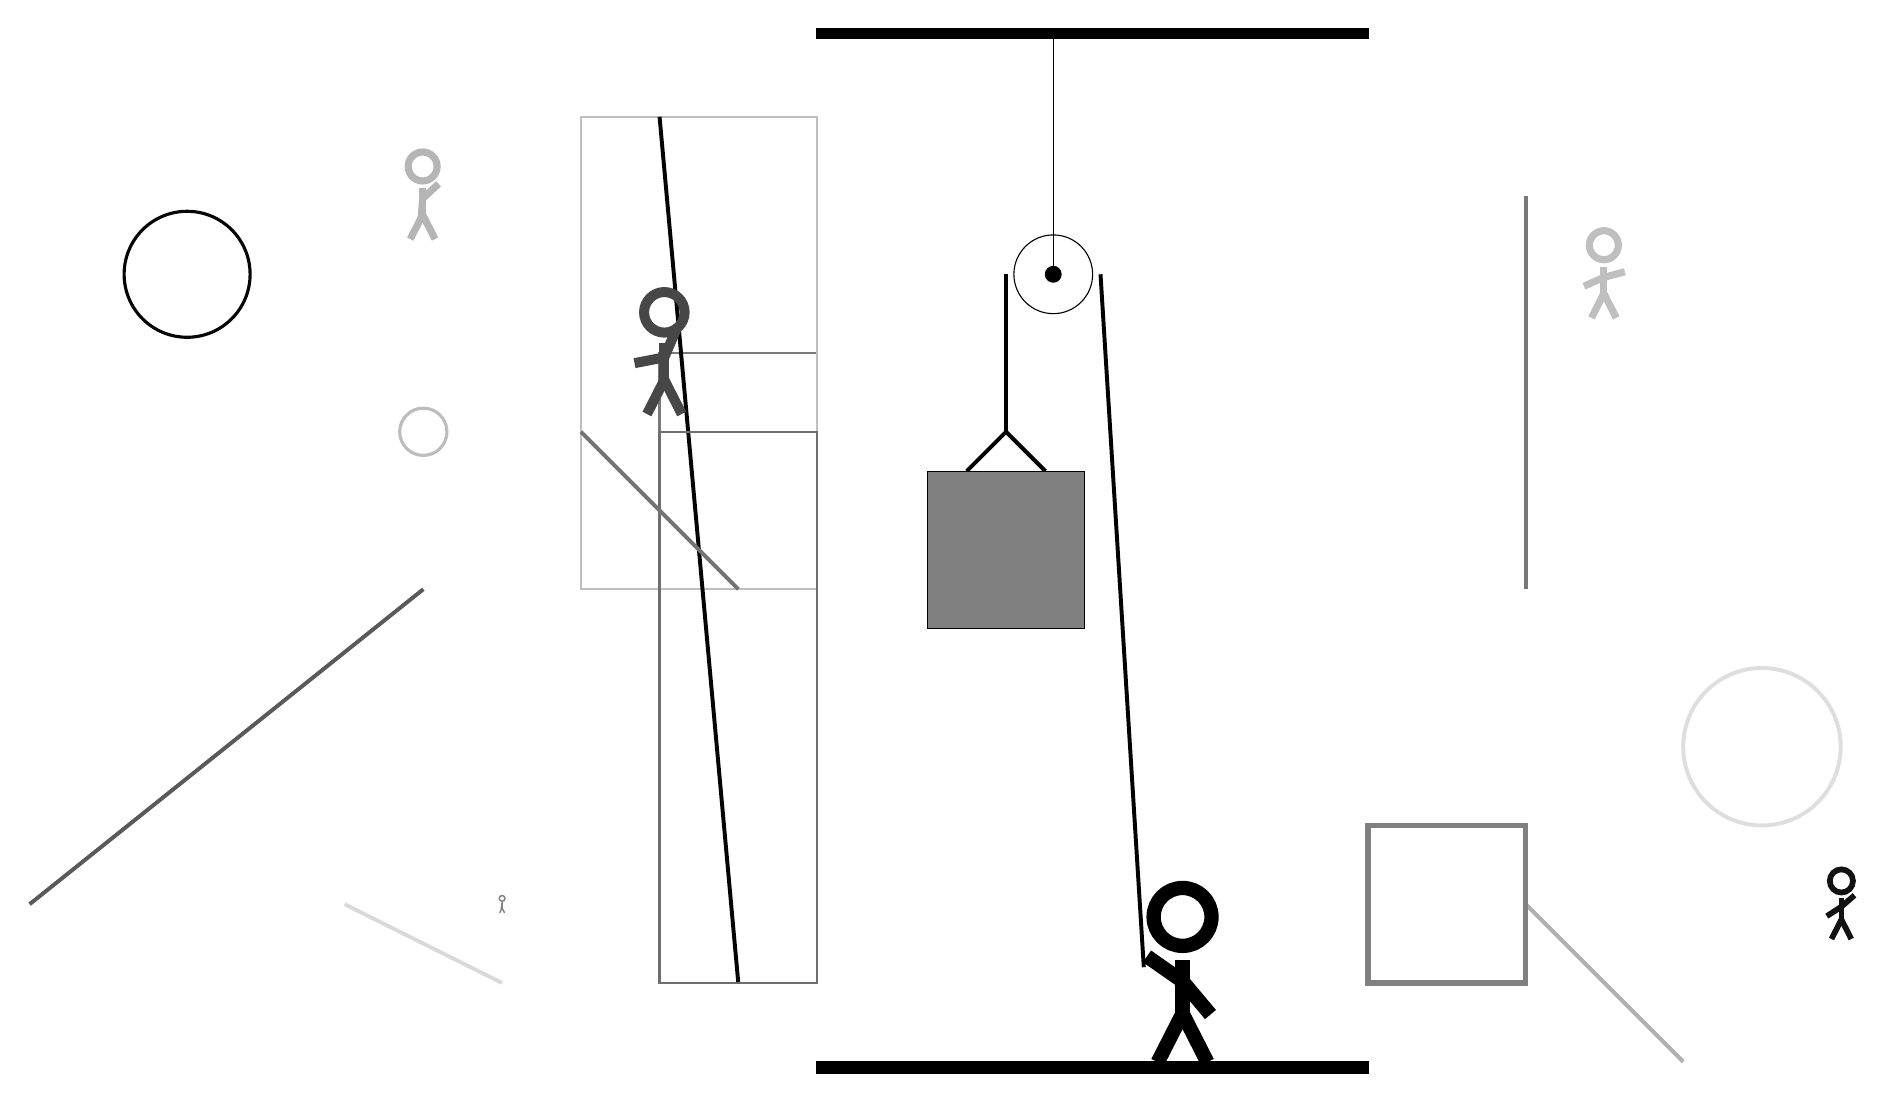
\begin{tikzpicture}
		%%%%% START %%%%%
		
		\draw[fill=black] (-2, 10) rectangle (5, 10.125);
		
		\draw (1, 7) circle (0.5);
		\draw[fill=black] (1, 7) circle (0.1);
		\draw (1, 10) -- (1, 7);
		
		\draw[line width=0.5mm] (-0.1, 4.5) -- (0.4, 5.0) -- (0.9, 4.5);
		\draw[fill=black!50] (-0.6, 4.5) rectangle (1.4, 2.5);
		
		\draw[line width=0.3mm, color=black!52] (-2, 6) rectangle (-4, -2);
		
		\draw [line width=0.4mm, color=black!26](-7, 5) circle (0.3);
		\node[line width=0.6mm, color=black!49] at (-6, -1) {\Strichmaxerl[1][77][84]};
		\node[line width=0.2mm, color=black!29] at (-7, 8) {\Strichmaxerl[5][86][43]};
		\draw[line width=0.5mm, color=black!31](7, -1) -- (9, -3);
		
		\draw[line width=0.5mm, color=black!15](-6, -2) -- (-8, -1);
		\draw[line width=0.5mm, color=black!53](7, 3) -- (7, 8);
		\draw[line width=0.3mm, color=black!25] (-2, 9) rectangle (-5, 3);
		\draw [line width=0.5mm, color=black!13](10, 1) circle (1.0);
		\node[line width=0.4mm, color=black!25] at (8, 7) {\Strichmaxerl[5][24][15]};
		
		\draw[line width=0.5mm, color=black!65](-7, 3) -- (-12, -1);
		
		\draw[line width=0.5mm, color=black!98](-3, -2) -- (-4, 9);
		\node[line width=0.6mm, color=black!93] at (11, -1) {\Strichmaxerl[4][33][41]};
		
		\draw[line width=0.7mm, color=black!50] (7, 0) rectangle (5, -2);
		\draw[line width=0.3mm, color=black!57] (-2, -2) rectangle (-4, 5);
		\draw[line width=0.5mm, color=black!55](-3, 3) -- (-5, 5);
		
		\draw[line width=0.5mm, color=black!87](10, 7) -- (10, 7);
		
		\draw [line width=0.4mm, color=black!98](-10, 7) circle (0.8);
		\node[line width=0.2mm, color=black!72] at (-4, 6) {\Strichmaxerl[7][11][67]};
		
		\draw[line width=0.5mm] (0.4, 7) -- (0.4, 5.0);
		\centerarc[line width=0.5mm](1, 7)(0:180:0.6);
		\draw[line width=0.5mm](1.6, 7) -- (2.15, -1.8);
		
		\node at (2.6, -1.9) {\Strichmaxerl[10][-35][-50]};
		
		\draw[fill=black] (-2, -3) rectangle (5, -3.15);
		
		%%%%% END %%%%%
	\end{tikzpicture}
\end{document}